\section{Ejercicio 7}
Los circuitos capaces de realizar operaciones aritméticas son pilares esenciales para la contrucción de distintos circuitos lógicos de aplicación. Mediante el uso de distintas compuertas es posible diseñar circuitos capaces de realizar la operación arimética más básica: la suma. Los contadores lógicos, son circuitos capaces de incrementar o decrementar de a un número. Existen basicamente dos tipos de contadores: los sincrónicos y los asincrónicos. La diferencia esencial entre ambos es que en los sincrónicos todos los elementos de memoria responden a un solo clock en simultáneo, mientras que los asincrónicos funcionan en cascada, lo que genera retrasos medibles en el cambio de estado del contador. 


Debido a que los flip flops que forman parte de los contadores se logran mediante la implementación correcta de transistores, los cambios de estado no son instantáneos. Se pueden definir distintos tiempos físicos que reflejan el comportamiento real de un flip-flop y de un contador o un circuito lógico en general. En primer lugar el tiempo de propagación o propagation delay time, en inglés, es el tiempo que le toma a la salida del circuito reflejar un cambio en la entrada, por ejemplo, un flanco positivo del clock. En segundo lugar, existen el tiempo de set-up y el tiempo de hold. El primero se refiere a cuanto tiempo antes de que ingrese un cambio en clock debe permanecer estable la señal entrante, mientras que el segundo es cuanto tiempo debo mantener dicho valor luego de aparecido el flanco de clock. Por último el rise y fall time, son los tiempos que le toma a la señal crecer desde un mínimo a un máximo y vicecersa. En general estos tiempos se toman desde el $10$ al $90$ porciento. Todas estas características son importantes para el funcionamiento de un contador ya que, de no controlarse pueden generarse glitches en el circuito. 

\subsection{Contador asincrónico} 

Una manera de implementar un contador que cuente hacia arriba es mediante el uso de flip flops tipo T. El siguiente circuito es un contador asincrónico de 3 bits, capaz de contar hasta 7. 

\begin{figure}[H]
	\centering
	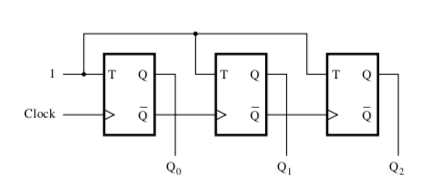
\includegraphics[width=0.8\textwidth]{Ejercicio7/Recursos/asincronico}
	\caption{Contador asincrónico}
\end{figure}

En el circuito se conectan los tres flip-flops en cascada, de ahí que sea asincrónico. La entradas de cada uno esta conectada a una señal constante igual a $1$, y por ende la salida de cada uno se invierte con cada falnco ascendente del Clock. Los últimos dos flip-flops están conectados a la salida $\bar{Q}$ correspondiente, por lo que cambian su estado siempre que la salida del anterior pase de $Q = 1$ a $Q = 0$, es decir un flanco positivo en $\bar{Q}$. Una desventaja clara de este tipo de circuitos es el delay de propagación. Debido a que los flip-flops están configurados en cadena, para obsrvar un cambio a la salida del último de ellos, la señal debe pasar por todos los anteriores, por ende habrá un retraso medible que hace poco práctica la implementación de este tipo de circuitos cuando se quiere contar grandes cifras. 


La máxima velocidad de operación del circuito, será entonces directamente dependiente del tiempo de propagación del mismo. 

%%Colocar tiempo de propagacion teorico, contando todas las compuertas involucradas.
%%Resultados y más discusion

\subsection{Contador sincrónico}

%%Dibujo circuito mas discusion funcionamiento.
%%Colocar tiempo de propagacion teorico, contando todas las compuertas involucradas.
%%Resultados y más discusion

\subsection{Mediciones}

\begin{table}[H]
\begin{tabular}{llll}\hline
\multicolumn{1}{c}{}           & \multicolumn{1}{c}{Hold time (ns)} & \multicolumn{1}{c}{Set-up time (ns)} & Propagation Delay (ns) \\
\hline
Contador asicr\'onico comercial ()    &                                &                                & $80-160$                  \\
Contador asincr\'onico implementado        &                                    &                                      &                        \\
Contador sincr\'onico comercial (MC14040) &                             &                          &                 \\
Contador sincr\'onico implementado   &                                    &                                      &                        \\  \hline
\end{tabular}
\end{table}

Es importante denotar que para el contador asincr\'onico el tiempo de propagaci\'on que brinda el fabricante es de la salida $Q_n$ a $Q_{n+1}$. 
\subsection{Conclusiones}

